\section{INTRODUCTION}

\afterpage{\begin{figure}[!t]
  \centering
  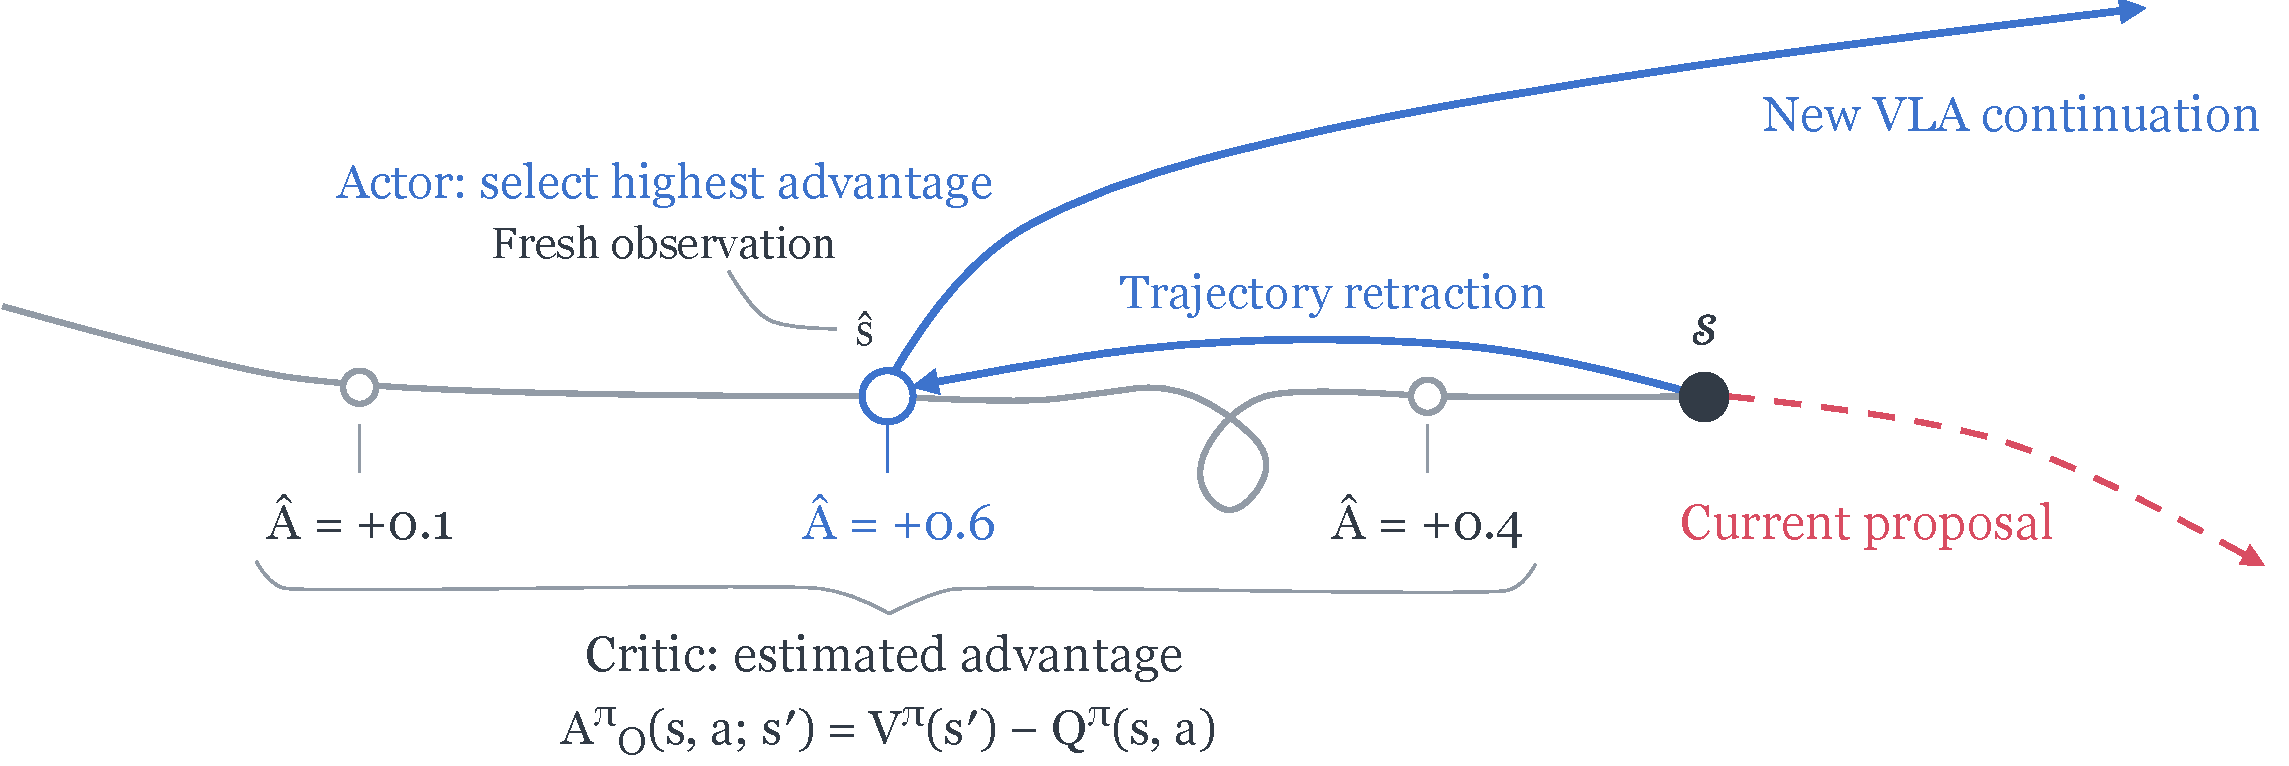
\includegraphics[width=\linewidth]{figures/acro-main-concept.pdf}
  \caption{\textbf{Actor--Critic rollout orchestration.} The orchestration advantage $A^\pi_{\mathcal O}(s,a;s')=V^\pi(s')-Q^\pi(s,a)$ compares task-success probabilities after re-entry and after executing the current proposal, within the available time. Once intervention is activated, the Actor selects the recorded candidate with the highest estimated advantage; the current $Q$ is fixed during this comparison. Trajectory Retraction shortens the return path, and the VLA resumes from a fresh observation.}
  \label{fig:acro-overview}
\end{figure}
}

Teaching a robot to act leaves open the question of when to trust its policy to continue and when to intervene. Vision-language-action (VLA) models map visual observations and language instructions to robot actions~\citep{zitkovich2023rt2,kim2025openvla,black2025pi0}. These models can succeed on a task in one execution and fail on the same task in another, suggesting that the outcome of a single execution may fall short of the policy's capabilities. Orchestration that translates this potential into successful task completion could improve the performance of an existing VLA without retraining the policy.


Effective orchestration requires two decisions: when to intervene, and how far that intervention should go. RoboMonkey and CoVer evaluate and select action proposals from the current observation~\citep{kwok2025robomonkey,kwok2026cover}, while AutoHorizon adjusts how much of a predicted action chunk to execute~\citep{wang2026autohorizon}. These decisions improve the policy's next execution, but evaluating an unfavorable proposal does not itself specify a physical intervention that would enable a better continuation. External orchestrators such as Pigey organize subgoals and skill calls, verify their outcomes, and apply retry and fallback rules~\citep{galanti2026pigey}. In Pigey's VLA interface, however, the orchestrator reassesses execution after a bounded rollout returns. Such verification and routing rules do not directly determine when to interrupt an ongoing VLA execution or how much to change its state before returning control. Intervening only as much as is useful requires evaluating the policy's prospects both if the current action proceeds and if execution resumes after an intervention.

We introduce ACRO, an Actor--Critic rollout orchestration layer that makes these decisions according to the deployed VLA's probability of task completion. ACRO learns action- and state-value estimates from execution outcomes. The Critic evaluates the VLA's proposed action to determine when to interrupt execution. To turn this assessment into a tractable intervention, we introduce \emph{Trajectory Retraction}, which reconstructs the observed execution path into a constrained region for intervention search. Within this region, ACRO uses state values to select a promising target reachable under the intervention budget. The Actor moves the robot to the selected configuration and returns control to the VLA, which observes the resulting state and generates a new continuation. Repeating this process within the remaining budget allows a minimal intervention layer to support alternative successful executions while leaving task execution to the existing policy.

We evaluate ACRO in simulation and on real-robot manipulation tasks. ACRO improves task success under the same execution budget, even when the physical steps used for trajectory retraction are included. These gains extend to the real robot, where success increases from $43.3\%$ to $65.0\%$. As the execution budget grows, ACRO achieves further gains in task completion, demonstrating test-time scaling through rollout orchestration.

Our contributions are as follows:
\begin{itemize}
\setlength{\itemsep}{2pt}
\item We formulate rollout orchestration through the difference in task-success probability between continuing a proposed action and resuming the policy after a physical intervention.
\item We introduce ACRO, which uses a shared Q/V Critic to decide when to intervene and Trajectory Retraction to select and reach a promising continuation point.
\item We show that ACRO improves success with fixed VLAs on SimplerEnv, RoboCasa, and real robots under matched physical execution budgets that include retraction.
\end{itemize}
